\documentclass[11pt]{article}
\usepackage[margin=1.5in]{geometry}
\usepackage{fontspec} % Advanced font selection
\setmonofont{Inconsolatazi4}
\usepackage{amsfonts, amsmath, amssymb, amsthm} % AMS Math Packages
\usepackage{mathtools} % Mathematical tools for amsmath
\usepackage{array, booktabs} % Extends the array and tabular environments
\usepackage{environ} % Interface for environments
\usepackage{parskip, setspace} % Paragraph indentation and line spacing
\usepackage{color} % Color control
\usepackage{colortbl} % Color to tables
\usepackage[x11names]{xcolor} % Color extensions 
\usepackage{soul} % Letter spacing, underlining, striking out 
\usepackage{hyperref} % Support for hypertext
\hypersetup{pdfborder=0 0 0, citebordercolor=Gray0, urlbordercolor=Gray0, linkbordercolor=Gray0}
\usepackage[capitalise]{cleveref} % Better cross-referencing
\usepackage{mdframed} % Framed environments that can split
\usepackage{fancybox, fancyhdr} % Variations of fbox and header/footer controls
\usepackage{tcolorbox} % Colored boxes 
\tcbuselibrary{breakable}
\usepackage{tabulary} % Tabular environments with variable width columns balanced
\usepackage{scrextend} % Extends KOMA-Script classes to standard classes
\usepackage{graphicx} % Enhanced support for graphics 
\usepackage[shortlabels]{enumitem} % Control layout of itemize, enumerate, description
\usepackage{tikz} % Graphics creation
\usetikzlibrary{shapes.geometric} 
\usepackage{fontspec, svg} % Include and extract SVG pictures
\usepackage[linesnumbered,lined,boxed,commentsnumbered]{algorithm2e} % Algorithms creation
\usepackage{listings} % Typeset source code listings
\usepackage{dcolumn} % Alignment on decimal points
\usepackage{float} % Improvements to floating objects
\usepackage[font=scriptsize,labelfont=bf]{caption}
\usepackage{pdflscape}
\usepackage{adjustbox}

\allowdisplaybreaks

\renewcommand{\baselinestretch}{1.25}
\sethlcolor{Cyan3!50}

\DeclarePairedDelimiter\floor{\lfloor}{\rfloor}
\DeclarePairedDelimiter\ceiling{\lceil}{\rceil}

\title{Section 1: Recurrences and Divide-and-Conquer Algorithms}
\date{January 26, 2024}
\author{Amy Zhao}

\begin{document}
\renewcommand\labelitemi{$\vcenter{\hbox{\tiny$\bullet$}}$}
\renewcommand\labelitemii{$\vcenter{\hbox{\tiny$\bullet$}}$}

\maketitle

\section{Recurrence Relations}
A \textbf{recurrence} is a description of a function in terms of itself which typically consists of one or more base cases and one or more recursive cases. A very common example is the Fibonacci recurrence relation. In the context of algorithms, these relations reflect the runtime of recursive algorithms. 

As a motivating example, consider the following function.

\IncMargin{2em}
\begin{algorithm}[H]
    \footnotesize
    \setstretch{1.125}
    \DontPrintSemicolon
    \SetKwProg{Fn}{Function}{:}{}
    \SetKwFunction{MysteryFunction}{MysteryFunction}
    \SetKwFunction{print}{print}
    \SetKwInOut{Input}{Input}\SetKwInOut{Output}{Output}
    \Fn{\MysteryFunction{$n$}}{
        \uIf{$n > 1$} {
            \print{``\upshape still going''}\;
            \MysteryFunction{$\frac{n}{2}$}\;
            \MysteryFunction{$\frac{n}{2}$}\;
        }
    }
\end{algorithm}\DecMargin{2em} 

Let $L(n)$ be the number of lines that the function above prints with input $n = 2^k$. For the base case $n = 1$ ($k = 0$), $L(1) = 0$; for $n = 2^k$ where $k \geq 1$, $L(n)$ satisfies:
\begin{equation}
    L(n) = 1 + 2L \left(\frac{n}{2}\right).
\end{equation}
When we write the first few values of $L(n)$, we can guess that $L(n) = n - 1 \equiv L(2^k) = 2^k - 1$ when $n = 2^k$. It's possible to prove this claim through induction. 

For the base case, we have $2^0 - 1 = 1 - 1 = 0$, which matches the solution $L(2^0) = L(1) = 0$ specified previously. In the inductive step, assume for any $k \geq 0$, $L(2^k) = 2^k - 1$ holds true. By definition of $L$, we have:
\begin{equation*}
    L(2^{k+1}) = 1 + 2L (2^{(k+1) - 1}) = 1 + 2L(2^k).
\end{equation*}
By the inductive hypothesis, we know $L(2^k) = 2^k - 1$, and we can make a substitution to the equation above:
\begin{equation*}
    L(2^{k+1}) = 1 + 2(2^k - 1)  = 1 + 2^{k+1} - 2 = 2^{k+1} - 1.
\end{equation*}
This proves the inductive step, which means the overall claim holds by the principle of induction. 

\subsection{The Master Theorem}
Recall that for divide and conquer algorithms, the runtime of the algorithm $T(n)$ is subject to the following inequality:
\begin{equation}
    T(n) \leq \underbrace{a \cdot T \left( \frac{n}{b} \right)}_{\substack{\text{work done by} \\ \text{recursive calls}}} + \underbrace{O(n^d)}_{\substack{\text{work done outside} \\ \text{recursive calls}}},
\end{equation}
where $a$ is the number of recursive calls, $b$ is the input size shrinkage factor, and $d$ is the exponent in the runtime of the ``combination step''.
\begin{center}
    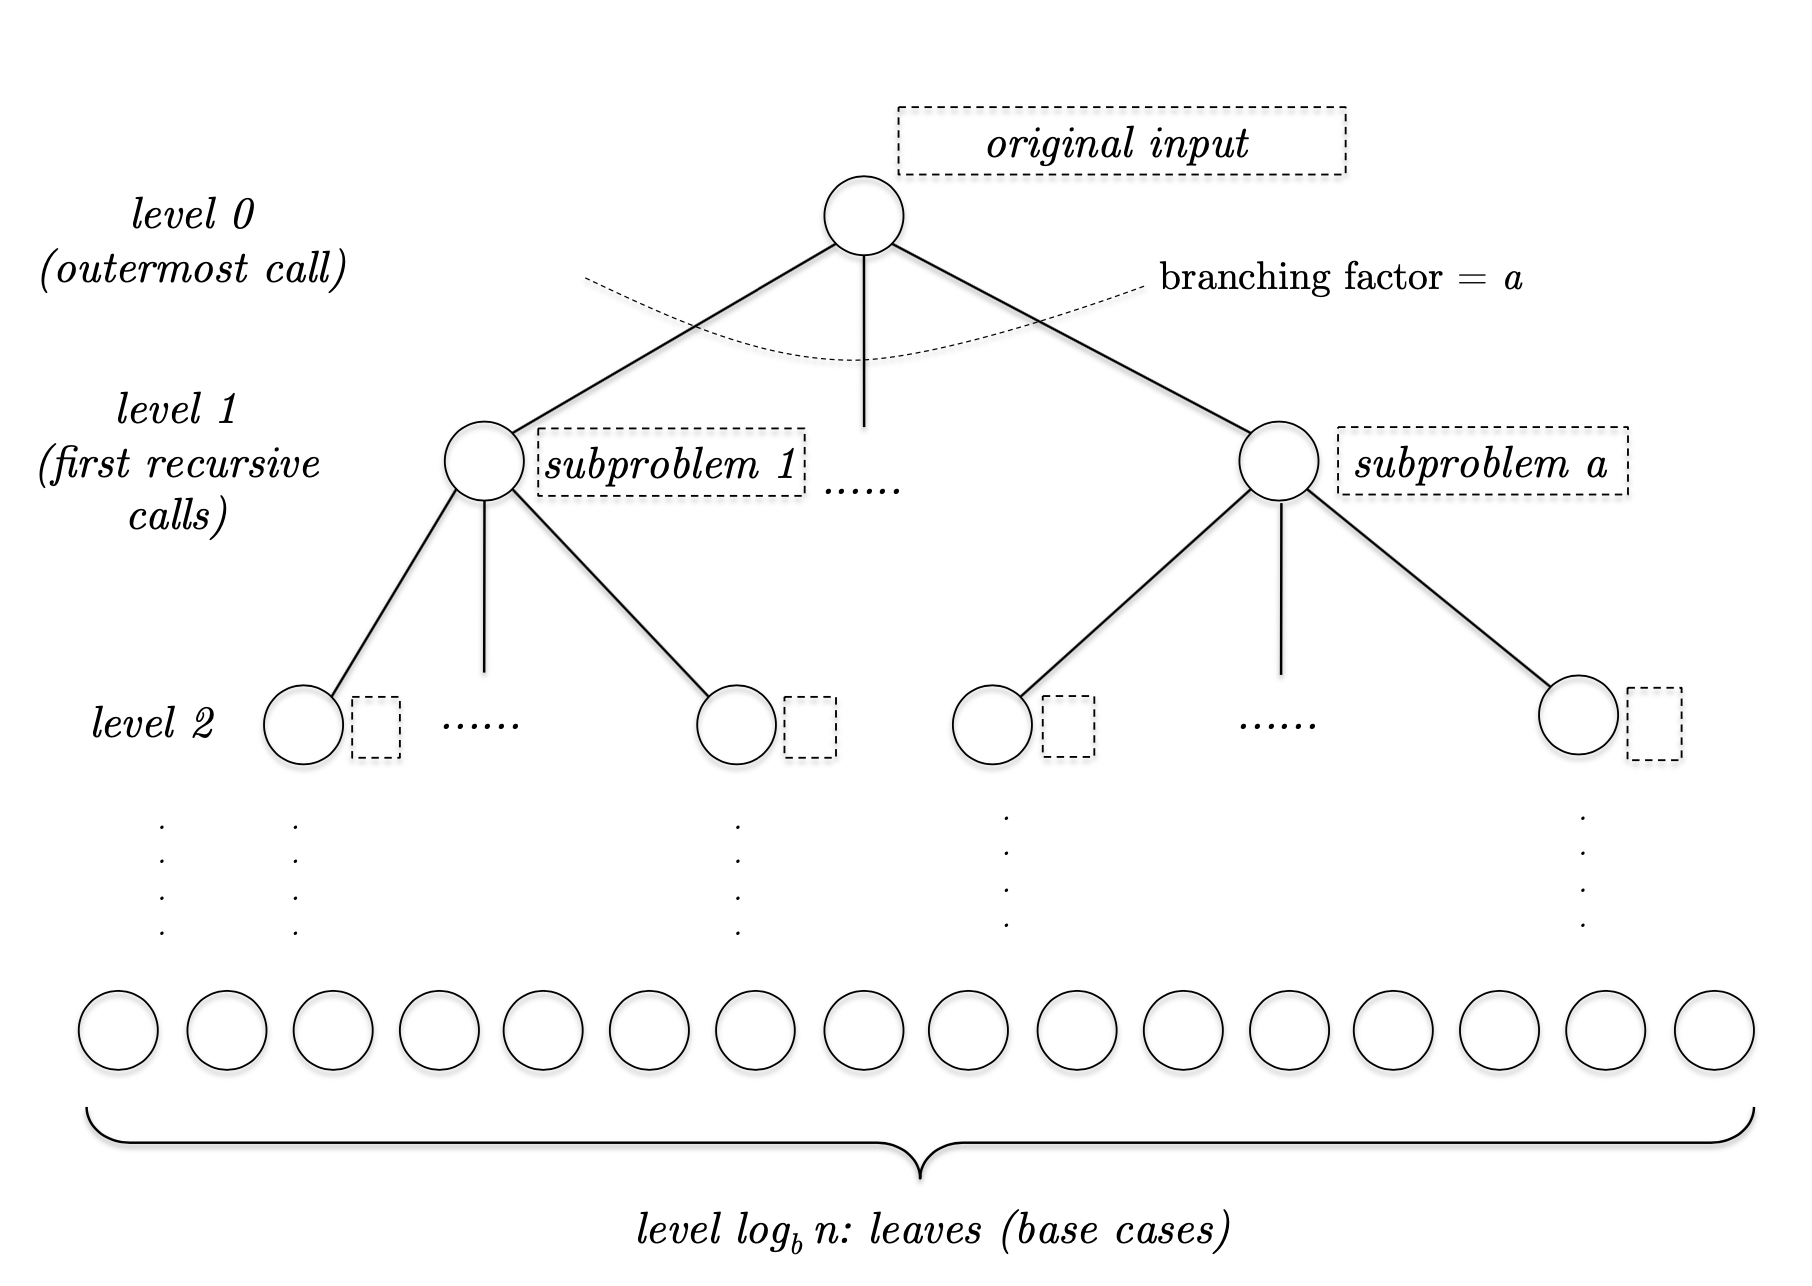
\includegraphics[width=0.7\textwidth]{figures/recursion_tree.png}
\end{center}
If $T(n)$ is defined by a standard recurrence, with parameters $a \geq 1$, $b > 1$, and $d \geq 0$, then 
\begin{gather} \label{MasterThm}
    T(n) = \begin{cases}
        O(n^d \log n) & \text{ if } a = b^d \\
        O(n^d) & \text{ if } a < b^d \\
        O(n^{\log_b a}) & \text{ if } a > b^d
    \end{cases}
\end{gather}
At a high level, the Master Theorem gives us a quick way to determine the runtime of a divide and conquer algorithm, provided we can identify the parameters $a$, $b$, and $d$. Keep in mind that not all recurrences apply to the Master Theorem. Some cases include when $a$ is a function of $n$; when there are not enough subproblems specified; and when the combination runtime is not positive.

To prove the Master Theorem, let $T(n) = a \cdot T \left(\frac{n}{b}\right) + O(n^d)$ be the recurrence we solve. Additionally, assume $T(1) = 1$ and that $n$ is a power of $b$ for simplicity. By applying the definition of big $O$, we have:
\begin{equation}
    T(n) \leq a \cdot T\left(\frac{n}{b}\right) + c n^d.
\end{equation}
In the recursion tree depicted above, there are $\log_b n + 1$ levels. At level $j$, there are $a^j$ subproblems, and each subproblem is of size $\frac{n}{b^j}$ which takes at most $c\left(\frac{n}{b^j}\right)^d$ time to solve. This implies that the total time required to complete level $j$ is at most $a^j \cdot c \left(\frac{n}{b^j}\right)^d = cn^d \left(\frac{a}{b^d}\right)^j$. Accounting for all levels, the runtime adheres to the following relationship:
\begin{equation}
    T(n) \leq cn^d \sum_{j=0}^{\log_b n} \left(\frac{a}{b^d}\right)^j.
\end{equation}
We now consider each of the three cases presented in \cref{MasterThm}:
\scriptsize 
\begin{equation}
    T(n) \leq \begin{cases}
        (\log_b n + 1)\cdot cn^d = O(n^d \log n) & \text{ if } a = b^d \\[1em]
        cn^d \sum_{j=0}^\infty \left(\frac{a}{b^d}\right)^j = cn^d \left(\frac{1}{1 - \frac{a}{b^d}}\right) = cn^d\left(\frac{b^d}{b^d - a}\right) = O(n^d) & \text{ if } a < b^d \\[1em]
        cn^d \left(\frac{\left(\frac{a}{b^d}\right)^{\log_b n + 1} - 1}{\frac{a}{b^d} - 1}\right) = O\left(n^d \left(\frac{a}{b^d}\right)^{\log_b n}\right) = O\left(n^d \cdot \frac{n^{\log_b a}}{n^d}\right) = O(n^{\log_b a}) & \text{ if } a > b^d
    \end{cases}
\end{equation}
\normalsize 

\subsubsection{Example}
Suppose you are choosing between the following three algorithms.
\begin{enumerate}
    \item Algorithm $A$ solves problems by dividing them into 5 subproblems of half the size, recursively solving each subproblem, and then combining the solution in linear time.
    \item Algorithm $B$ solves problems of size $N$ by recursively solving two subproblems of size $n - 1$ and then combining the solutions in constant time. 
    \item Algorithm $C$ solves problems of size $n$ by dividing them into nine subproblems of size $\frac{n}{3}$, recursively solving each subproblem, and then combining the solutions in $O(n^2)$ time. 
\end{enumerate}
The recurrence for each algorithm and the resultant time complexity is defined below:
\begin{align*}
    A: \text{ } & T(n) = 5T\left(\frac{n}{2}\right) + O(n) \Longrightarrow O(n^{\log_2 5}) = O(n^{2.33})\\
    B: \text{ } & T(n) = 2T(n - 1) + O(1) \Longrightarrow O(2^n) \\
    C: \text{ } & T(n) = 9T\left(\frac{n}{3}\right) + O(n^2) \Longrightarrow O(n^2\log n) 
\end{align*}
Thus, algorithm $C$ has the quickest runtime among the three algorithms.

\section{Loop Invariants}
In order to prove correctness for divide and conquer algorithms, we introduce the notion of a loop invariant. A \textbf{loop invariant} is a condition that is true at the beginning and end of every iteration of a loop. Proofs involving loop invariants are analogous to proofs by induction. In the base case (initialization), we show that the loop invariant is true before beginning the loop. In the inductive step, we show that if the loop holds over some number of iterations, it must hold over the next iteration as well. When the loop exits, the algorithm should output the correct answer because the loop invariant has held. 

One key difference between a proof by loop invariant and a proof by induction is that the inductive step is applied finitely (until the loop terminates), as opposed to the indefinite application of the inductive step in regular mathematical induction. An example of this proof style is presented in the following sections, contrasted with a more traditional induction proof. 

\section{Divide and Conquer Algorithms}
Any problem which requires a divide and conquer algorithm can be split into three primary steps.
\begin{enumerate}
    \item Divide the input into smaller subproblems. 
    \item Solve the subproblems recursively. 
    \item Combine the solutions for the subproblems into a solution for the original problem. 
\end{enumerate}
To apply these steps, a common approach is to first start with the entire input data and make a comparison of two values. Depending on the results of this comparison, we determine which portion of the input data to recurse on. 

\subsection{Binary Search}
Binary search is one of the most common examples of divide and conquer you might encounter. The goal of binary search is to find the index of a target element by search the appropriate half of a sorted array, determined by comparing the middle element to the target element. If the target value is less than the middle value, the algorithm continues on the lower half. If the target is greater than the middle element, the algorithm continues on the upper half. 

\IncMargin{2em}
\begin{algorithm}[H]
    \footnotesize
    \setstretch{1.125}
    \DontPrintSemicolon
    \SetKwData{Left}{left}\SetKwData{This}{this}\SetKwData{Up}{up}
    \SetKwProg{Fn}{Function}{:}{}
    \SetKwFunction{BinarySearch}{BinarySearch}
    \SetKwInOut{Input}{Input}\SetKwInOut{Output}{Output}
    \Input{Sorted array $A$ of $n$ elements and a target $T$}
    \Output{Index of $T$ if it exists; $-1$ otherwise}
    \BlankLine
    \Fn{\BinarySearch{$A$, $n$, $T$}}{

        $L \gets 0$, $R \gets n - 1$ \;
        \BlankLine
        \While{$L \leq R$}{
            $m \gets \lfloor \frac{L + R}{2} \rfloor$\;
            \BlankLine
            \uIf{$A[m] < T$}{$L \gets m + 1$}
            \uElseIf{$A[m] > T$} {$R \gets m - 1$}
            \uElse{\Return{$m$}}
        }
        \Return{$-1$}
    }
\end{algorithm}\DecMargin{2em} 

To prove correctness, we first consider the initialization of the loop. The array $A$ is given as a sorted array, and the array remains sorted because the loop doesn't shuffle the. When the length of the list is at least $n = 1$, then we have $0 \leq L \leq R \leq n - 1$. We also know that the target index is definitely between $L$ and $R$ if the target exists. 

Suppose $L'$ and $R'$ represent the values of $L$ and $R$ at the end of the loop. We want to show that if the invariant is true at the beginning of the loop body, it must hold at the end of the loop as well. $m$ is the average of $L$ and $R$, so it must be that $L \leq m \leq R$. The execution of the remaining portion of the loop depends the value of $A[m]$, so there are a couple of cases to consider. 
\begin{itemize}
    \item $A[m] < T$: In this case, we shift our search to the ``upper'' half of the array. $L' = m + 1$ and $R' = R$. Since $A$ is sorted, the target element must exist after the element $A[m]$ in the list, and we can safely discard the ``lower half''. We maintain the relationship of $L' \leq R' \leq n - 1$ (assuming that the loop continues to another iteration).
    \item $A[m] > T$: In this case, we shift our search to the ``lower'' half of the array. $L' = L$ and $R' = m - 1$. Since $A$ is sorted, the target element must exist before the element $A[m]$ in the list, and we can safely discard the ``upper half''. We maintain the relationship of $L' \leq R' \leq n - 1$ (assuming that the loop continues to another iteration).
    \item $A[m] = T$: We have found the index of the target element to return ($m$), and it is safe to terminate the loop. 
\end{itemize}
If no iteration encounters the third case listed, then the target element doesn't exist in the array, and the loop eventually encounters the case where $L > R$. The algorithm accounts for this correctly by returning $-1$.

The recurrence for binary search is:
\begin{equation}\label{BinSearch}
    T(n) = T \left(\frac{n}{2}\right) + O(1),
\end{equation}
as each recursive call divides the search space in half, and there is only constant time work done outside of the recursive calls. This means that $a = 1$, $b = 2$, and $d = 0$, corresponding to a runtime of $O(n^0 \log n) = O(\log n)$. 

\subsubsection{Recursive Binary Search}
Unsurprisingly, there is a recursive algorithm for binary search as well.

\IncMargin{2em}
\begin{algorithm}[H]
    \footnotesize
    \DontPrintSemicolon
    \setstretch{1.125}
    \SetKwProg{Fn}{Function}{:}{}
    \SetKwFunction{RecursiveBinarySearch}{RecursiveBinarySearch}
    \SetKwInOut{Input}{Input}\SetKwInOut{Output}{Output}
    \Input{Sorted array $A$ of $n$ elements, target $T$}
    \Output{Index of $T$ if it exists; $-1$ otherwise}
    \Fn{\RecursiveBinarySearch{$A$, $n$, $T$}} {
        \uIf{$n = 1$} {
            \uIf{$T = A[1]$} {
                \Return{$1$}\;
            } 
            \uElse{\Return{$-1$}}
        } \Else{
            $m \gets \floor*{\frac{n}{2}}$\;
            \uIf{$T < A[m]$} {
                \Return{\RecursiveBinarySearch{$A[1:m]$, $T$}}
            } \uElseIf{$T > A[m]$}{
                \Return{\RecursiveBinarySearch{$A[m + 1:n]$, $T$}}
            } \uElse{
                \Return{$m$}
            }
        }
    }
    \BlankLine
\end{algorithm}\DecMargin{2em} 
To prove correctness, let $P(n)$ be the predicate which is true if the algorithm works on any sorted array $A$ of length $n$ and target $T$. We wish to prove $\forall n \in \mathbb{N}: P(n)$. For the base case, we consider $P(1)$. If $T$ is indeed in the array, then it must be that $T = A[1]$. If $T$ is not in the array, we return $-1$, which is the desired result. In both cases, the algorithm behaves properly. 

In the inductive step, first fix a natural $k \in \mathbb{N}$. Suppose the predicate is true for all $\ell$ such that $1 \leq \ell \leq k$. In other words, $P(1), P(2), \dots, P(k)$ are all true, and we wish to prove $P(k + 1)$. For notation purposes, set $N = k + 1$. We first handle the case where the target $T$ does not exist in array $A$, which implies $T \neq A[m]$ regardless of the value of $m$. Furthermore, we have $T \notin A[1:m]$ and $T \notin A[m + 1:N]$. Both $A[1:m]$ and $A[m + 1:N]$ have lengths $\floor*{\frac{N}{2}}$ and $\ceiling*{\frac{N}{2}}$, so these subarrays are covered by the inductive hypothesis. Thus, the algorithm will return $-1$.  

The other case occurs when $T \in A$; it follows that there is some index $1 \leq j \leq N$ such that $T = A[j]$. If $j = m$, the algorithm correctly returns $m$. If $j < m$, we have that $T = A[j] < A[m]$ because the array is sorted, and the recursive call on line 10 will run. Here, $m = \floor*{\frac{N}{2}} < N$, so the recursive call will return the correct index under the inductive hypothesis. If $j > m$, we have that $T = A[j] > A[m]$ because the array is sorted, and the recursive call on line 12 will run. $A[m + 1: N]$ has length $\ceiling*{\frac{N}{2}} < N$, so the recursive call will return the correct index for $T$. 

\subsection{Repeated Squaring}
Given two integers $a$ and $n$, we would like to compute $a^n$. The direct method that computes $a^n$  by performing $n$ multiplications of $a$ is computationally inefficient for large inputs. It turns out that we can implement a divide and conquer approach. 

\IncMargin{2em}
\begin{algorithm}[H]
    \footnotesize
    \DontPrintSemicolon
    \setstretch{1.125}
    \SetKwProg{Fn}{Function}{:}{}
    \SetKwFunction{Power}{Power}
    \SetKwInOut{Input}{Input}\SetKwInOut{Output}{Output}
    \Input{Base $a$ and exponent $n$}
    \Output{Result of $a^n$}
    \BlankLine
    \Fn{\Power{$a$, $n$}}{
        \uIf{$n = 0$}{\Return{1}}
        \uElseIf{$n$ is even}{
            $k \gets$ \Power{$a$, $\frac{n}{2}$}\;
            \Return{$k \cdot k$}
        }
        \uElse{
            $k \gets$ \Power{$a$, $\frac{n - 1}{2}$}\;
            \Return{$k \cdot k \cdot a$}
        }
    }
\end{algorithm}\DecMargin{2em} 
To analyze the time complexity, we solve the following recurrence for $n \geq 1$:
\begin{align}
    \begin{split}
        T(n) &\leq T\left(\floor*{\frac{n}{2}}\right) + 2 \\
        &\leq T\left(\floor*{\frac{n}{4}}\right) + 2 + 2 \\
        &\leq \cdots \leq T(1) + \underbrace{2 + \cdots + 2}_{\log_2(n) \text{ copies}} \leq 2 \log_2(n).       
    \end{split}
\end{align}
This implies that the algorithm runs in $O(\log n)$ time. We could alternatively apply the Master Theorem; there is one recursive call per iteration, and the ``input'' size is divided in half. The recurrence mirrors the one presented for binary search, \cref{BinSearch}.

\subsection{Maximum Sum of Subarray}
Suppose we want to design a divide and conquer algorithm to find the value of the maximum sum of any subsequence of array $A$. As an example, input $A = [2, 1, -1, 3, -1, -2, 3]$ should output $5$ because the subsequence which produces the maximum sum is $[2, 1, -1, 3]$. The main idea is to split $A$ into two parts of equal length and find the maximum sum subsequence of each part, as well as the maximum sum that passes through both partitions. We set $A_L = A[1 : \floor*{\frac{n}{2}}]$ and $A_R = A[\floor*{\frac{n}{2}} + 1: n]$; $M_L$ is the maximum sum subsequence of $A_L$, and $M_R$ is the maximum sum subsequence of $A_R$. 

Let $N_L$ be the maximum subsequence of $A_L$ that ends with the last element of $A_L$. We can compute this by starting from the last element and iterating backward over the elements of $A_L$. For each element encountered, we add it to a running sum and determine if we have a ``new'' maximum sum. Similarly, let $N_R$ be the maximum sum subsequence of $A_R$ that starts with the first element of $A_R$. We can compute $N_R$ by iterating over the elements of $A_R$ in the forward direction and tracking the running sum and maximum sum. The sum $N = N_L + N_R$ represents the maximum sum subsequence of $A$ that passes through both portions of $A$. The maximum sum subsequence of $A$ is simply the maximum value of the three sums calculated, $M = \max \{M_L, M_R, N\}$.

\IncMargin{2em}
\begin{algorithm}[H]
    \setstretch{1.125}
    \footnotesize
    \DontPrintSemicolon
    \SetKwProg{Fn}{Function}{:}{}
    \SetKwFunction{MaxSum}{MaxSum}
    \SetKwFunction{LeftSum}{LeftSum}
    \SetKwFunction{RightSum}{RightSum}
    \SetKwInOut{Input}{Input}\SetKwInOut{Output}{Output}
    \Input{Array $A$ with length $n$}
    \Output{Maximum sum of a subsequence}
    \BlankLine
    \Fn{\LeftSum{$A$, $n$}} {
        $S \gets 0$ \tcp*{used to track sum of $A[i : n]$}
        $N \gets -\infty$ \tcp*{used to track max sum of $A[i : n]$}
        \BlankLine
        \For{$i = n$ to $i = 1$}{
            $S \gets S + A[i]$ \; 
            $N \gets \max\{N, S\}$\;
        }
        \BlankLine
        \Return{N}
    }
    \BlankLine
    \Fn{\RightSum{$A$, $n$}} {
        $S \gets 0$ \tcp*{used to track sum of $A[1 : i]$}
        $N \gets -\infty$ \tcp*{used to track max sum of $A[1 : i]$}
        \BlankLine
        \For{$i = 1$ to $i = n$}{
            $S \gets S + A[i]$\; 
            $N \gets \max\{N, S\}$ \;
        }
        \BlankLine
        \Return{$N$}
    }
    \BlankLine
    \Fn{\MaxSum{$A$, $n$}}{
        \uIf{$n = 1$}{
            $M \gets A[1]$\;
        }
        \uElse{
            $A_L \gets A \left[1 : \frac{n}{2}\right]$\;
            $A_R \gets A \left[\frac{n}{2} + 1 : n\right]$\;
            $M_L \gets$ \MaxSum{$A_L$, $\frac{n}{2}$}\;
            $M_R \gets$ \MaxSum{$A_R$, $\frac{n}{2}$}\;
            $N_L \gets$ \LeftSum{$A_L$, $\frac{n}{2}$}\;
            $N_R \gets$ \RightSum{$A_R$, $\frac{n}{2}$}\;
            $N \gets N_L + N_R$ \; 
            $M \gets \max\{M_L, M_R, N\}$\;
        }
        \Return{$M$}
    }
\end{algorithm}\DecMargin{2em} 
For a given array $A$ of size $n$, we make two recursive calls on input sizes $\frac{n}{2}$. Finding the maximum subarray that crosses the midpoint takes $O(n)$ time. The time complexity can thus be expressed as the following recurrence relation:
\begin{equation}
    T(n) = 2T \left(\frac{n}{2}\right) + O(n), 
\end{equation}
which yields a time complexity of $O(n \log n)$ by the Master Theorem.
\end{document}